%-------------------------------------------------------------------------------
%	PACKAGES EN DOCUMENT CONFIGURATIE
%-------------------------------------------------------------------------------

\documentclass[hidelinks]{uva-inf-article}

\usepackage[style=numeric-comp]{biblatex}
\addbibresource{PT-essay.bib}
\usepackage{listings}

\setlength{\parindent}{0em}
\setlength{\parskip}{1em}

\usepackage{float}

\usepackage{tikz}
\usetikzlibrary{arrows.meta}
\usetikzlibrary{positioning}
\tikzset{
    >={Latex[width=2mm,length=2mm]},
    base/.style =   {
                        rectangle, rounded corners, draw=black,
                        minimum width=4cm, minimum height=1cm,
                        text centered, font=\sffamily
                    },
    start_stop/.style = {base, fill=black, text=white},
    loading/.style = {base, fill=orange!15},
    analyse/.style = {base, fill=red!15},
    optimize/.style = {base, fill=blue!15},
    generate/.style = {base, fill=green!15}
}

%-------------------------------------------------------------------------------
%	GEGEVENS VOOR IN DE TITEL
%-------------------------------------------------------------------------------

% Vul de naam van de opdracht in.
\assignment{Pre-Masters Programme Software Engineering}
% Vul het soort opdracht in.
\assignmenttype{Essay}
% Vul de titel van de eindopdracht in.
\title{CiviC Compiler Report}

% Vul de volledige namen van alle auteurs in.
\author{René Kok}
\uvanetid{13671146}

\author{Aram Mutlu}
\uvanetid{13574116}

% Vul eventueel ook de naam van de docent of vakcoordinator toe.
\docent{Dhr. dr. C.U. Grelck}
\course{Compiler Construction}
% Te vinden op onder andere Datanose.
\courseid{5062COMP6Y}

% Dit is de datum die op het document komt te staan. Standaard is dat vandaag.
\date{\today}

%-------------------------------------------------------------------------------
%	VOORPAGINA
%-------------------------------------------------------------------------------

\begin{document}
\maketitle
\newpage

%-------------------------------------------------------------------------------
%	INHOUDSOPGAVE EN ABSTRACT
%-------------------------------------------------------------------------------

\tableofcontents
\begin{abstract}
\end{abstract}
\newpage

%-------------------------------------------------------------------------------
%	INTRODUCTIE
%-------------------------------------------------------------------------------
\section{Introduction}
\par This report documents the CiviC compiler we build in 
the course Compiler Construction by dr. C.U. Grelck. The goal of the CiviC compiler 
is to create a CiviC compiler that transforms CiviC code into CiviC assembly code 
that a computer can understand. In this report we will focus on different aspects 
of our compiler and what we did and how we did it. We will do this by following the order of the milestones,
from scanning/parsing to code generation and also use the milestones to further 
explain the compiler. Unfortunately, we did not implement any of the extensions and optimizations beyond the standard 
milestones for a functional compiler.

%-------------------------------------------------------------------------------
%	METHODE
%-------------------------------------------------------------------------------
\newpage
\section{The compiler}
\begin{figure}[H]
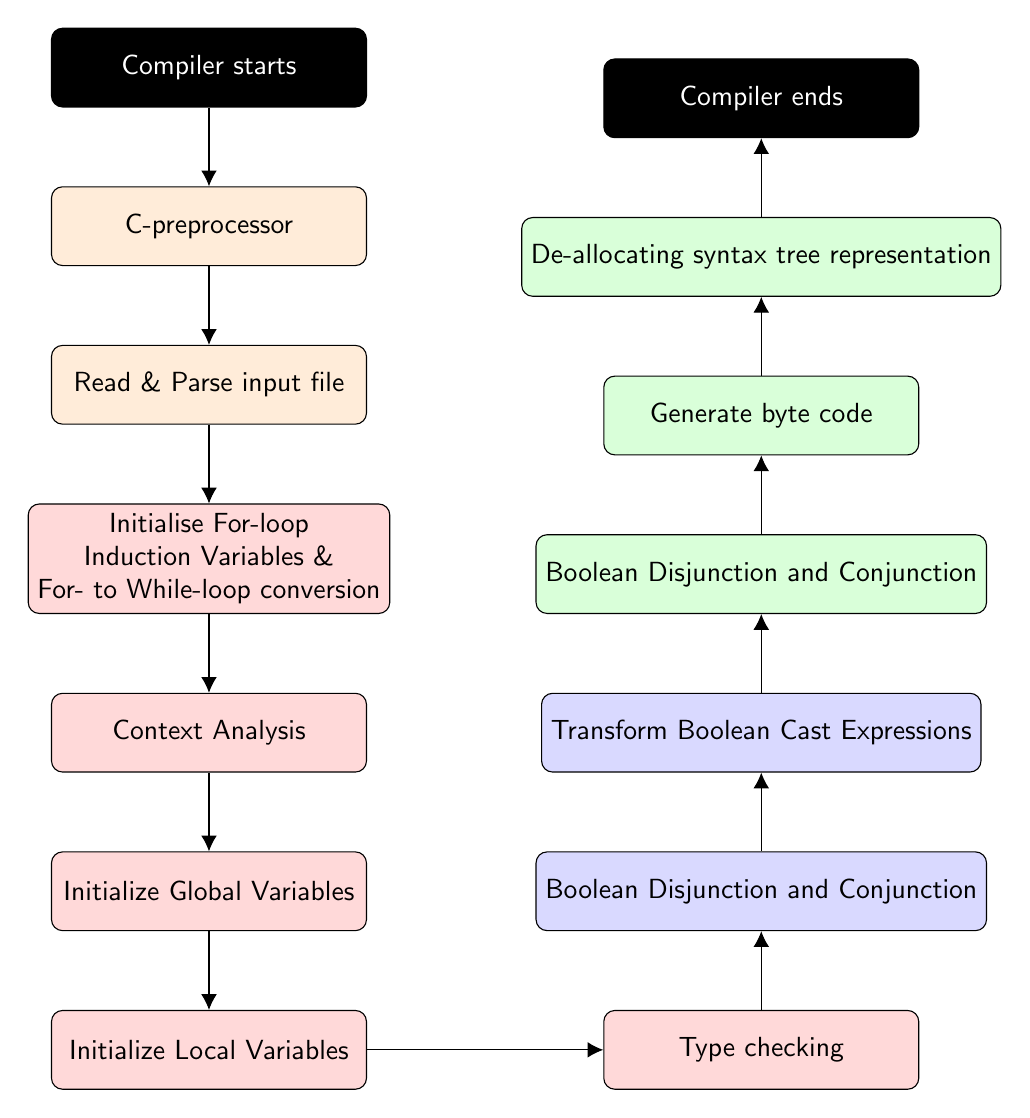
\begin{tikzpicture}[node distance=1cm and 3cm, every node/.style={fill=white, font=\sffamily}, align=center]
    \node (start)             [start_stop]              {Compiler starts};

    \node (c_preprocessor)     [loading, below=of start]          {C-preprocessor};    
    \node (read_input_file)     [loading, below=of c_preprocessor]          {Read \& Parse input file};    
    
    \node (for_loop)     [analyse, below=of read_input_file]          {Initialise For-loop \\ Induction Variables \& \\ For- to While-loop conversion};  
    \node (context_analyse)     [analyse, below=of for_loop]          {Context Analysis};  
    \node (init_globals)     [analyse, below=of context_analyse]          {Initialize Global Variables};  
    \node (init_locals)     [analyse, below=of init_globals]          {Initialize Local Variables};  
    \node (type_checking)     [analyse, right=of init_locals]          {Type checking}; 
    
    \node (bool_dis_con)     [optimize, above=of type_checking]          {Boolean Disjunction and Conjunction}; 
    \node (bool_cast)     [optimize, above=of bool_dis_con]          {Transform Boolean Cast Expressions}; 

    \node (print_ast)     [generate, above=of bool_cast]          {Boolean Disjunction and Conjunction}; 
    \node (gen_bytec)     [generate, above=of print_ast]          {Generate byte code}; 
    \node (frtr)     [generate, above=of gen_bytec]          {De-allocating syntax tree representation}; 

    \node (ActivityEnds)      [start_stop, above=of frtr] {Compiler ends};

    \draw[->]             (start) -- (c_preprocessor);
    \draw[->]             (c_preprocessor) -- (read_input_file);
    \draw[->]             (read_input_file) -- (for_loop);
    \draw[->]             (for_loop) -- (context_analyse);
    \draw[->]             (context_analyse) -- (init_globals);
    \draw[->]             (init_globals) -- (init_locals);
    \draw[->]             (init_locals) -- (type_checking);
    \draw[->]             (type_checking) -- (bool_dis_con);
    \draw[->]             (bool_dis_con) -- (bool_cast);
    \draw[->]             (bool_cast) -- (print_ast);
    \draw[->]             (print_ast) -- (gen_bytec);
    \draw[->]             (gen_bytec) -- (frtr);
    \draw[->]             (frtr) -- (ActivityEnds);
\end{tikzpicture}
\caption{A schematic overview of our compiler}
\label{fig:ThCoStep1}
\end{figure}

\par See Figure 1 for a schematic overview of our compiler. The steps we have implemented are respective explained in the next chapters. 
Steps that are not covered are: c-preprocessor reading input file and de-allocating syntax tree representation, 
these were already provided by the framework. 
The reason why we, unfortunately, convert a for- to while-loop so early on is discussed in our reflection.
Each color in the diagram represents a different phase as described in the compiler (phase.mac file). 
Orange is the Loading CiviC program phase, red is the semantic analysis phase, 
purple is the code optimizer phase and green is the final code generating phase.

\newpage
\subsection{Lexicographic Analysis}
The first step for building a CiviC compiler is to create (or extend in this case) 
the scanner that reads the CiviC code (stream of characters) that recognizes the 
symbols and words and outputs a (finite) stream of tokens.
By recognizing the words and symbols the Scanner can use pattern matching to find see
what the next action will be for the compiler. For the scanner to know which symbols
are available in the CiviC language, we need to define these ourselves. We did this 
by defining all the possible symbols (parenthesis, brackets and binary operators etc.)
which are supported by the CiviC language. The CiviC language only supports integers,
floats and booleans so there is no need to define other types in the compiler.

In our scanner we added a validator that validates if an integer is too large or too small by 
comparing it to the max int and min int. We included the "limits.h" file in our civic.l
to get the values of the min and max range of an integer. If the integer is too high or too low the compiler
returns an CTIerror telling the integer is out of range.

\begin{lstlisting}[basicstyle=\small, language=C, label=lst:code-1, caption=Integer range check, captionpos=b]
[0-9]+ { 
            long integer = strtol(yytext, NULL, 10);
            if (integer < INT_MIN || integer > INT_MAX) {
                CTIerrorLine(yylineno, "Integer %s out of range", yytext);
            }
            yylval.cint=atoi(yytext);
            FILTER( INTVAL);
        }
\end{lstlisting}

After completing the scanner we needed to refine our intermediate representation (abstract
syntax tree) for our compiler. We used the AST that was provided by the course and added some 
elements of our own. To make the SymbolTable work properly we added the SymbolTable node to the
AST along with the SymbolTableEntry. A SymbolTableEntry contains all the information about 
an entry such as in which SymbolTable its stored in, name, type, if its a function/parameter/export,
its offset, depth and its definition. We did the same for the CodeGenTable and the CodeGenTableEntry.
The CodeGenTableEntry stores information for a single line of code generation such as the
index, instruction and the value of the generated code. Code generation will be further 
explained in section 6 of this report.

To properly illustrate the logical structure of the code we had to expand the print traversals
to cover the full syntactic range of the CiviC language. Each node in the AST has its own
print traversal which prints the information of the specific node in the Print AST phase.

\newpage
\subsection{Syntatic Analysis}
After the scanner is done and creates a (finite) stream of tokens, the parser comes
into play and will start its job. The parser will use the output from the scanner and
use it to create and output an abstract syntax tree (AST). The parser uses the stream 
of tokens to do pattern matching with the pre defined casus in the compiler. 

The parser does all the pattern matching for us. For each node in the AST we created 
a new node with its pattern in civic.y so the parser can match them. The civic.y is a
YACC file which stands for "Yet Another Compiler Compiler” and auto-generates parsers
from context-free grammars. The YACC file contains all patterns with their corresponding
actions to perform.

Listing 2 shows a simple example of pattern matching. In this example we added the
node with its pattern so the pattern matching visible. 

\begin{lstlisting}[basicstyle=\small, language=C, label=lst:code-2, caption=Pattern matching Example, captionpos=b]
int b;          // globdef: type ID SEMICOLON

void foo() {    // fundef: type ID PARENTHESIS_L PARENTHESIS_R  CURLY_L
                    // funbody (inside curly brackets)
    int a = 2;      // vardecl: type ID LET expr SEMICOLON
    b = 1;          // assign: varlet LET expr SEMICOLON (varlet: ID)
}               // CURLY_R 
\end{lstlisting}

At the end of the civic.y YACC file we added an error function that prints an error message
with CTIabort so the user can see where the error came from (line + col number) and what
the error message is. 

\subsection{Initialise For-loop Induction Variables \& For- to While-loop conversion}
Transforming for- into while-loops will be done after the analyzing phase. The compiler checks
for for-loops in the syntax tree and will replace them with semantically equivalent while-loops.
The first step is to declare the for-loop variables (start, stop, step) and then use these 
variables to create the new while loop. If we use a simple for-loop like:

\begin{lstlisting}[basicstyle=\small, language=C, label=lst:code, caption=For-loop example, captionpos=b]
m=5;
for(int i=10,m,-1)
{
        printInt(i);
}
\end{lstlisting}

\newpage
As input in the compiler we would get the following while-loop:

\begin{lstlisting}[basicstyle=\small, language=C, label=lst:code, caption=While-loop example, captionpos=b]
_for_1_i = 10;
_for_1_i_stop = m;
_for_1_i_step = -1;
while ((( _for_1_i_step > 0 ) ? ( _for_1_i < _for_1_i_stop ) 
        : ( _for_1_i > _for_1_i_stop )))
{
    printInt(_for_1_i);
    _for_1_i = ( _for_1_i + _for_1_i_step );
}
\end{lstlisting}

In the example above we can see the while-loop the compiler created. It first checks if the step is greater
than zero. If this is true checks if the counter is less then de stop, if so -> execute body while-loop. If
the step is not greater than zero, it will check of the counter is greater than the stop. If this is true it 
will execute the body of the while loop.

\subsection{Context Analysis}
Semantic Analysis consists of 2 parts: the context analysis and the type checker. The context
analyser uses the output from the parser (the AST) and adds an initial symbol table to the AST.
The type checker validates the given code. For example, he validates whether the correct 
types are used in assign statements or whether methods return the correct type.

The context analyser stores an pointer to the current symbol table in a custom info struct created for the context analyser.
This pointer is necessary because we need to know to which symbol table we want to add a new entry while performing the context analysis.
A global symbol table is added to the program node.
In this global table, global declarations and definitions and function declarations and definitions are stored.
A new symbol table is created for each function declaration and definition. 
This table is attached to the relevant symbol table entry by means of a child node.
A new info struct is created in which the symbol table pointer points to this new table. 
With this info struct, the statements of the function are traversed. 
Because the info struct now refers to the function's symbol table, the new symbol table entries are added to this table.

\newpage
\subsection{Turning Variable Initialisations into Regular Assignments}
Milestone 6: Turning Variable Initialisations into Regular Assignments, is done in two different traversals.
global- and local\_variable\_initialisation.c. 
In both files, the declaration and initialization are separated for the respective variables types.

\subsubsection{Global variable initialisation}
Global variable initialization works by creating an "\_\_init" function. 
This function is the first function definition added to the program node, after which the rest of the programs' function definition and function declarations follows.
A pointer to this init function is included in the info struct so that it is possible to request the init function in other methods.
After the initialization function has been created, the other declarations of the program are traversed.
If a declaration node is a global definition, the initialization statement is disconnected and moved to the init function.
This init function will later also be used by the CiviC-VM.

\begin{lstlisting}[basicstyle=\small, language=C, label=lst:code-3, caption=Output of global variable initialisation, captionpos=b]
export void __init (  ) 
{
        a = 321;
        b = 1.000000;
        c = false;
}

export int a;
export float b;
export bool c;
\end{lstlisting}

\subsubsection{Local variable initialisation}
The declaration and initialization of local variables is done in the function definition.
For every function in a program, the body function is traversed. 
When the traversal encounters a variable definition, it disconnects the initialization and a new initialization statement is created for that variable.
This initialization statement is added after all variables are declared but before the rest of the function's expressions are executed.

\begin{lstlisting}[basicstyle=\small, language=C, label=lst:code-4, caption=Output of local variable initialisation, captionpos=b]    
export int foo() 
{
    int a;
    int b;
    a = 128;
    b = 64;
    return a + b;
}
\end{lstlisting}

\newpage
\subsection{Type Checking}
The type checker traverse through the output of the context analyser (the AST with symbol tables) 
to check all the types and their values. The output of the type checker is the AST with the symbol table.
Our type checker validates if a function's return statement returns the right type, 
if a called function is declared in the code, if a binary operator is used with two compatible types, 
if a value can be casted to the given type and if an variable declaration is initialized with the corresponding type.

\subsection{Optimiser}
% Milestone 9, 10 
The next step in the compiler is the optimiser. The optimiser replaces code with "better" code
than the original. By doing this it will improve the execution speed, code size end energy
consumption. The new code that replaced the old code is always semantically equivalent to the 
original code.

% Milestone 9
\subsubsection{Compiling Boolean Disjunction and Conjunction}
Short circuit boolean evaluation cannot be mimicked by special VM instructions alone. The standard 
compiler approach is to systematically replace disjunction and conjunction operators by semantically 
equivalent if-then-else constructs. But because this is very challenging we got recommended to use the
C ternary operator pred?then:else. We created a file called bool\_disjunction.c that handles these 
code transformations. The file checks if the binary operator is an "\textbar \textbar" (or) or is if its an "\& \&" (and).
Because each of these operators has a different effect on the outcome of the ternary operator. For 
the "\textbar \textbar" operator it will use the left operator (BINOP\_LEFT(...)) as the "pred" in the ternary operator,
use TRUE as the "then" and right operator as the "else". For the "\&\&" operator it will be the other way 
round because both left- and right operators need to be checked. The left operator will be the "pred",
the right operator will be used as the "then" and the "else" will be a FALSE.

% TODO: Milestone 10
\subsubsection{Compiling Boolean Cast Expressions}
The CiviC language features cast expressions to convert values between all three basic types, possibly 
with loss of precision. The CiviC-VM, however, only has conversion instructions between integer numbers 
and floating point numbers and vice versa. We needed to implement a compiler pass for the systematic 
transformation of cast expressions with Boolean argument or result value into semantically equivalent 
non-cast expressions. We added a new sub phase "Transform Boolean Cast Expressions" which calls the 
TBCtransformBooleanCast in the transform\_boolean\_cast.c file which traverses through the syntax tree.
If it comes across a cast it wil first check what cast type it is, if its a bool it will then check if the
variable is an Int of Float and then replace the arg\_node with a new binary operator. If the cast type
is not a bool it will check if the info type is a bool, if this is true we need to cast the boolean to 
either an Int or a Float. By checking the cast type of the node we can assign the corresponding ternary
to the arg\_node the same way like the short circuit boolean evaluation explained in the previous paragraph.

\newpage
\subsection{Code Generation}
\par The last stage of the compiler, the bytecode generation, is converting the abstract syntax tree into assembly code. 
With this assembly code, the virtual machine specially designed for Civic can execute the given Civic code.

\par The whole code generation is done in a single traversal named "Generate byte code".
The default traversal mode of the code generation is set to "user", because almost all nodes are traversed.
There are a few code generation methods that do nothing, and immediately return the node. 
These methods were necessary because without these methods the compiler would not compile because the user specified traversal expects one method for each AST node.

\par A special code generation table and code generation table entry has been designed for saving and printing the global variables, constants, imports and exports. 
The code generation table consists of 4 child nodes in which these instructions are stored.

\par Generating the bytecode is done in a fairly simple way.
The abstract syntax tree is traversed and based on certain flags and attributes and of the different 
nodes instructions are printed and/or added to the correct code generation table.
After the AST has been traversed and the main instructions have been printed, the global variables, constants, 
imports and exports instructions (which are stored in the code generation table) are printed.
The byte code is exported to stdout by default, but it is also possible to export the output of the compiler to any given file.
We made the choice for printing to stdout so debugging would be easier. 

\newpage
\section{Reflection}
\par Besides the fact that we had little prior knowledge of how a compiler worked, the entire language c was also new to us.
We programmed with Java and Python before, but c was completely new. This made building a compiler a bit more difficult.

The milestone we have been working on the longest was getting our parser in order.
The civic.y at one point gave around 200 shift/reduce conflicts. Eventually, after 2,5 weeks and about 3 TA-sessions we were able to resolve our problems with the parser.
In addition, the end results of milestones (such as milestone 6) were sometimes very unclear. Fortunately, the TAs were always very enthusiastic and helpful when you came up with questions. 
After a TA session we often thought: "Oh was that it?" Milestones often sounded more difficult than they actually were.
Another problem that took us too much time to solve was the '.importfun' instruction while generating the byte code. 
We got the following error after running the test files: "error: Unable to find 'printInt' in any of the modules". 
This was due to the fact that we did not include the parameters in the functionSignature of the pseudo instruction '.importfun'. 
It took us a whole day to finally find this 'simple' bug, and was then resolved within 5 minutes.
We expected that generating byte code would be a lot harder than it ended up being. 
We had this assumption mainly because the scope of this traversal encompasses the entire Civic program/source code supplied and because bytecode was initially 
incomprehensible to us. This turned out not to be the case afterwards, partly due to the clearly supplied CiviC-VM specification.

Something we are not too happy about in our compiler is that the last week before creating the compiler, we found out that there was no for-loop instruction in the Civic VM. 
Unfortunately, this resulted in a quick and dirty method of converting a for-loop to while-loop in the traversal that was meant to declare the induction variables of the for-loops 
(for\_loop\_variable\_initialisation.c). 
We had chosen for this solution with the idea of eventually doing this in a separate specific traversal, 
but due to time constraints, this never happened.

All in all, we are very satisfied with our end result. 
We have managed to write a working compiler that at least passes all the basic checks provided. 
We are very proud that we have accomplished this in a period of about 8 to 10 weeks. 
We had learned during the open day that this course was one of the toughest of the program.

What we regret is that we did not have enough time to work on the extensions. 
We started the course with the idea to also work on the extensions, but due to a lack of time,
because we were also following the programming languages course in addition to Compiler construction, this was not successful.
Because there are all kinds of hurdles involved, implementing arrays sounded very interesting.
From what we can remember from the first lesson about publishing and sharing our compiler, 
we regret that this is not allowed. We think that making this compiler is one of the prestigious projects we have made so far. 
Writing a compiler has been compared to fighting a dragon for a reason.

\end{document}